\begin{frame}{La deuda neta se mantendría cerca de 59\% del PIB}
\centering
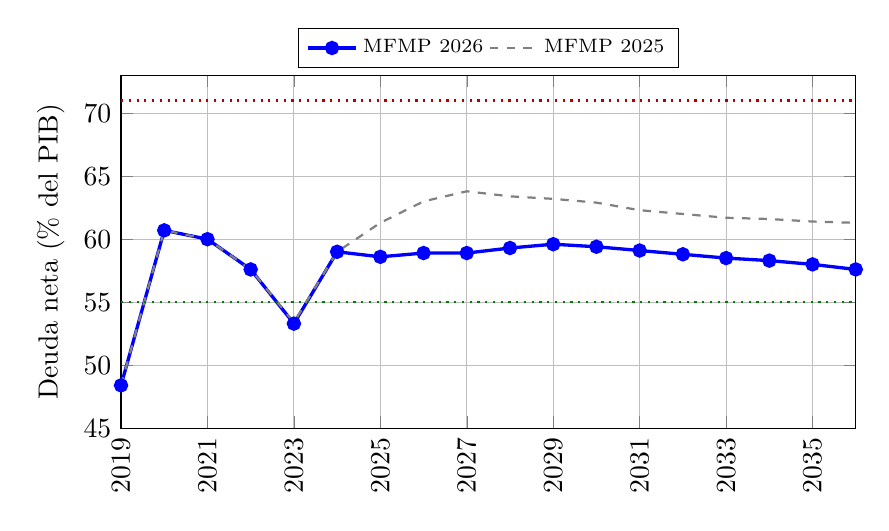
\begin{tikzpicture}
\begin{axis}[
  width=0.90\textwidth,height=0.50\textwidth,
  ylabel={Deuda neta (\% del PIB)},xmin=2019,xmax=2036,ymin=45,ymax=73,
  xtick={2019,2021,...,2035},xticklabel style={rotate=90,anchor=east,/pgf/number format/.cd,1000 sep={},fixed,precision=0},scaled x ticks=false,
  ytick={45,50,...,70},grid=major,
  legend style={at={(0.5,1.02)},anchor=south,legend columns=2,font=\scriptsize}
]
\addplot[color=blue,very thick,mark=*] coordinates {
 (2019,48.4) (2020,60.7) (2021,60.0) (2022,57.6) (2023,53.3) (2024,59.0)
 (2025,58.6) (2026,58.9) (2027,58.9) (2028,59.3) (2029,59.6) (2030,59.4)
 (2031,59.1) (2032,58.8) (2033,58.5) (2034,58.3) (2035,58.0) (2036,57.6)
};
\addlegendentry{MFMP 2026}
\addplot[color=gray,dashed,thick] coordinates {
 (2019,48.4) (2020,60.7) (2021,60.0) (2022,57.6) (2023,53.4) (2024,59.0)
 (2025,61.3) (2026,63.0) (2027,63.8) (2028,63.4) (2029,63.2) (2030,62.9)
 (2031,62.3) (2032,62.0) (2033,61.7) (2034,61.6) (2035,61.4) (2036,61.3)
};
\addlegendentry{MFMP 2025}
\addplot[color=red!70!black,dotted,thick] coordinates {(2019,71) (2036,71)};
\addplot[color=green!50!black,dotted,thick] coordinates {(2019,55) (2036,55)};
\end{axis}
\end{tikzpicture}

\scriptsize Fuente: MFMP 2026, capítulo 3, gráfico 3.10. La línea gris muestra la senda publicada en el MFMP 2025.
\end{frame}